\section{\review{Beam Instrumentation}}


% ============================================
%          Beam Position Monitors
% ============================================
\subsection{\review{Beam Position Monitors}}

Beam Position Monitors (BPMs) are one of the most utilized and essential elements of beam 
diagnostics in particle accelerators. In the LHC, most of the BPMs are dual plane, and thus composed
of four electrodes, distributed as two per plane. The BPM system consists of over than 550 BPMs pear
beam, distributed along the ring, in the arcs and the IPs. The most common type, the
\textit{curved-button}, shown in \cref{fig:beam_instrumentation_bpm_button}, is typically placed
near quadrupoles~\cite{wendt_bpm_2020}.

\begin{figure}[H]
    \centering
    \begin{subfigure}[b]{0.45\textwidth}
        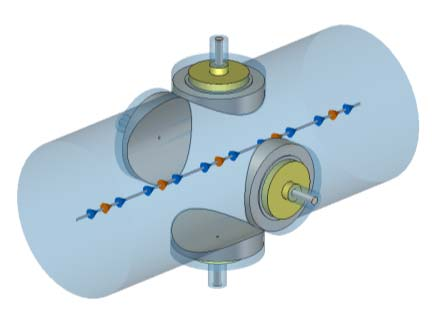
\includegraphics[width=\textwidth]{images/lhc_bpm_button.jpg}
        \caption{Button \textit{"BPM"} type BPM of the LHC~\cite{wendt_bpm_2020}.}
        \label{fig:beam_instrumentation_bpm_button}
    \end{subfigure}
    \hfill
    \begin{subfigure}[b]{0.45\textwidth}
        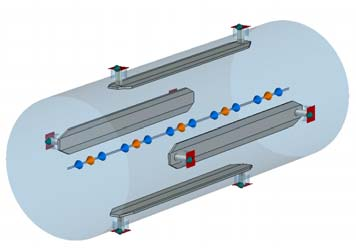
\includegraphics[width=\textwidth]{images/lhc_bpm_stripline.jpg}
        \caption{Stripline \textit{"BPMSW"} type BPM of the LHC~\cite{wendt_bpm_2020}.}
        \label{fig:beam_instrumentation_bpm_stripline}
    \end{subfigure}
\end{figure}

Other pickups such as the \textit{stripline}, shown in
\cref{fig:beam_instrumentation_bpm_stripline}, albeit more complex and expensive, offer a better
signal to noise ratio and are capable of identifying the direction of the
beam~\cite{wendt_bpm_2020}. Such features are essential for the LHC, were both beams travel through
the same aperture at the IPs.\\ 
The BPM response is not linear with the beam position, which requires a post-processing not
systematically implemented in accelerators beam diagnostics systems. LHC's BPMs have been simulated
and polynomials fitted to minimize this response error~\cite{a_nosych_geometrical_2014}.


 
% ============================================
%                Collimators
% ============================================
\subsection{\review{Collimators}}

Collimators are a crucial part of the LHC. Their purpose is to protect the machine against beam
losses and clean the outer parts of the beam~\cite{redaelli_lhc_2011}. The energy of the beams in
the LHC is high enough to not only quench the magnets, but to also damage the elements.

At injection energy, with a low intensity pilot bunch, the consequences of a loss are though less
severe. During Run 3, in 2022, a new collimator sequence was introduced, making a safe exploitation
of the machine possible with more retracted collimators. This made measurements with higher kick
amplitudes and larger orbit offsets, and thus momentum offsets, possible.


% ============================================
%             Beam Loss Monitors
% ============================================
\subsection{\review{Beam Loss Monitors}}

Beam Loss Monitors are detectors mounted on various elements of the accelerator, such as magnets or
collimators, to detect abnormal losses of particles. They play a crucial role in the protection of
the machine, triggering a dump when losses exceed the threshold set for their respective element. 
BLMs use ionization chambers, working on the same principle as simple Geiger counters: a tube filled
with gas, in presence of a high voltage.

Dashboards in the control room are regularly used to monitor the losses along the ring when
performing optics measurements, as those prove to often be destructive.

% ============================================
%                 AC-Dipole
% ============================================
\subsection{\review{AC-Dipole}}

The AC dipole of the LHC is a crucial component for optics studies. Its primary function is to
excite the beam into large coherent oscillation, achieved by applying a sinusoidally oscillating
dipole field~\cite{miyamoto_parametrization_2008}. By ramping up and down adiabatically the field,
large coherent oscillations can be produced without any decoherence or emittance growth.
\Cref{fig:ac_dipole} shows an example of a measurement made with an AC-Dipole.  Exciting the beam to
large amplitudes make the study of linear optics, such as beta-beating easier, and that of non
linear optics such as resonances possible.

\begin{figure}
    \center
    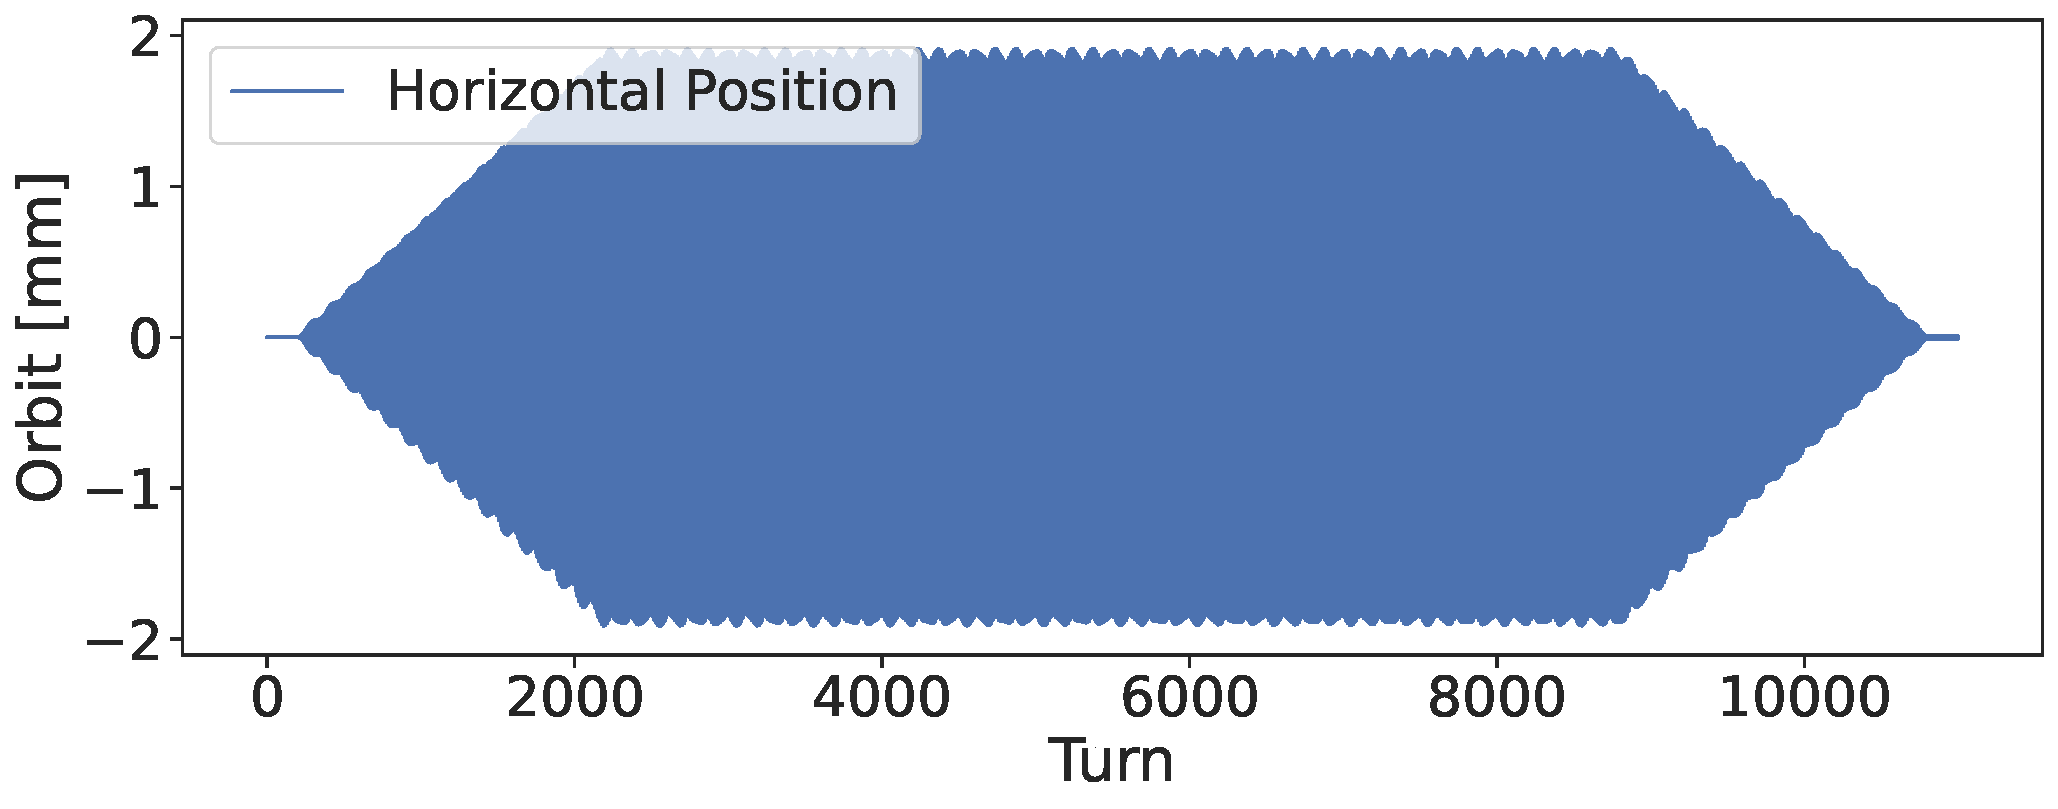
\includegraphics[width=0.9\textwidth]{./images/ac_dipole_tbt.pdf}
    \caption{Simulated turn by turn data with an AC-Dipole first ramping up then down.} 
    \label{fig:ac_dipole}
\end{figure}

The AC-Dipole is set to oscillate at a frequency $Q_d$, different from the natural tune of the
machine $Q$ and thus introduces systematic effects that needs to be compensated during the optics
analysis. The new orbit of a particle under the influence of the AC-Dipole, at turn number $n$ and
observation point $s$, is given by~\cite{serrano_lhc_2010}:

\begin{equation}
z(s, n) = \frac{BL}{4\pi\rho\delta_z} \cdot \sqrt{\beta_z(s) \beta_{z,0}} \cdot \cos \left( 2 \pi Q_{d,z}n + \phi_z(s) + \phi_{z,0}\right),
\label{eq:ac_dipole}
\end{equation}

where $B$ is the amplitude of the oscillating magnetic field, $L$ the length of the AC-Dipole,
$B\rho$ the magnetic rigidity, $\delta$ the difference between $Q_d$ and $Q$, $\beta$ and $\beta_0$
the beta function at the observed point and the AC-Dipole, $\phi$ and $\phi_0$ the phase advance at
the observed point and of the AC-Dipole.